% Report.
%
% Copyright (C) 2010  Vladimir Rutsky <altsysrq@gmail.com>
%
% This work is licensed under a Creative Commons Attribution-ShareAlike 3.0 
% Unported License. See <http://creativecommons.org/licenses/by-sa/3.0/> 
% for details.

% TODO: Use styles according to GOST (it's hard).

\documentclass[a4paper,10pt]{article}

% Encoding support.
\usepackage{ucs}
\usepackage[utf8x]{inputenc}
\usepackage[T2A]{fontenc}
\usepackage[russian]{babel}

\usepackage{amsmath, amsthm, amssymb}

% Indenting first paragraph.
\usepackage{indentfirst}

\usepackage{url}
\usepackage[unicode]{hyperref}

%\usepackage[final]{pdfpages}

\usepackage[pdftex]{graphicx}
\usepackage{subfig}

%TODO: use texments
\usepackage{listings}

\newcommand{\HRule}{\rule{\linewidth}{0.5mm}}

% Spaces after commas.
\frenchspacing
% Minimal carrying number of characters,
\righthyphenmin=2

% From K.V.Voroncov Latex in samples, 2005.
\textheight=24cm   % text height
\textwidth=16cm    % text width.
\oddsidemargin=0pt % left side indention
\topmargin=-1.5cm  % top side indention.
\parindent=24pt    % paragraph indent
\parskip=0pt       % distance between paragraphs.
\tolerance=2000
%\flushbottom       % page height aligning
%\hoffset=0cm
%\pagestyle{empty}  % without numeration

\newcommand{\myemail}[1]{%
\href{mailto:#1}{\nolinkurl{#1}}}

\begin{document}

% Title page.
% title.tex
% Report title page.
% Copyright (C) 2010  Vladimir Rutsky <altsysrq@gmail.com>

\begin{titlepage} % начало титульной страницы

\begin{center} % включить выравнивание по центру

\large Санкт-Петербургский государственный политехнический университет\\[5.5cm]
% название института, затем отступ 5,5см

\huge Отчет по курсовой работе\\[0.6cm] % название работы, затем отступ 0,6см
\large по~курсу <<Верификация программ>>\\[1cm]
\large <<Разработка контроллера светофоров на перекрёстке и его верификация>>\\[6cm]
% тема работы, затем отступ 6см

\begin{flushright} % выровнять её содержимое по правому краю
\begin{tabular}{l l}
Студент: & Руцкий~В.\,В.\\
Группа: & 5057/2\\
Вариант: & 9, 13\\
Преподаватель: & Шошмина~И.\,В.
\end{tabular}
\end{flushright} % конец выравнивания по правому краю

\vfill % заполнить всё доступное ниже пространство

{\large Санкт-Петербург 2010}
\end{center} % закончить выравнивание по центру
\thispagestyle{empty} % не нумеровать страницу
\end{titlepage} % конец титульной страницы


\tableofcontents
\pagebreak

% Content

\section{Постановка задачи}
Задан автомобильный перекрёсток, его конфигурация показана на рис.~\ref{fig:crossroad} (вариант 9, 13).
\begin{figure}[h!]
  \centering
  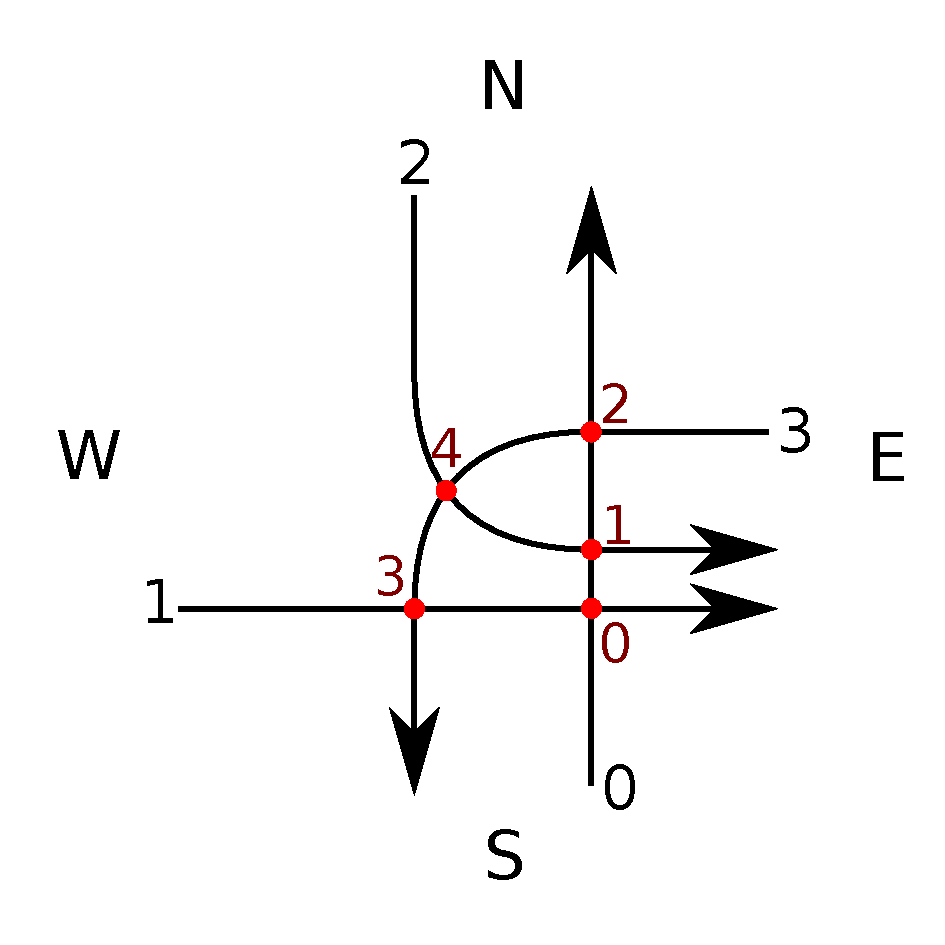
\includegraphics[width=0.5\linewidth]{./data/crossroad.pdf}
  \caption{Схема перекрёстка}
  \label{fig:crossroad}
\end{figure}
На перекрёстке возможны следующие направления движения транспорта:
\begin{itemize}
  \item $\mathrm{S} \rightarrow \mathrm{N}$,
  \item $\mathrm{W} \rightarrow \mathrm{E}$,
  \item $\mathrm{N} \rightarrow \mathrm{E}$,
  \item $\mathrm{E} \rightarrow \mathrm{S}$.
\end{itemize}
Каждое направление движения регулируется собственным светофором.
На каждом направлении движения установлены датчики, фиксирующие наличие автомобилей.

При отсутствии автомобилей на полосе, соответствующий светофор должен гореть красным светом.
При появлении машин на полосе, соответствующий светофор должен убедиться, 
что по всем полосам, пересекающим текущую, движение транспорта запрещено 
(их светофоры горят красным), и загореться зелёным светом, пропуская машины.
При наличии машин на различных полосах, светофоры должны периодически переключаться, 
обеспечивая равномерный пропуск машин по всем направлениям.

Требуется разработать модель управления данным светофором на языке \textit{Promela}, 
удовлетворящую указанным выше требованиям, 
и верифицировать её корректность с помощью пакета \textit{Spin}%
\footnote{\url{http://www.spinroot.com/}}.

\section{Решение}

\subsection{Моделирование внешней среды}
Внешняя среда в данной задаче моделируется процессами \textit{LineTrafficGenerator}, 
см.~код~\ref{src-traffic-generator} (полный текст исходных кодов приведён в приложении~\ref{appendix-sources}).
В качестве датчиков, фиксирующих присутствие автомобилей, 
выступает массив каналов \textit{carsWaiting}~--- по одному каналу на каждый светофор.

Автомобили генерируются недетерминированно. 
Для каждого направления создаётся новый процесс \textit{LineTrafficGenerator},
отвечающий за генерацию машин, движущихся через соответствующий светофор.

\lstinputlisting[language=Promela,numbers=left,%
firstline=53,firstnumber=53,lastline=69,%
caption={Моделирование внешней среды},%
label=src-traffic-generator]{data/main.pml}

\subsection{Моделирование светофоров}
Каждый светофор моделируется процессом \textit{TrafficLight}, см.~код~\ref{src-traffic-lights}.

При своей работе светофор хранит своё состояние (цвет) в глобальном массиве \textit{tlColor} 
(строка~115).

Светофор зависит от общих ресурсов~--- пересечений полос движения: 
чтобы безопасным образом включить зелёный свет на светофоре, необходимо,
чтобы на всех светофорах, пути которых пересекают путь данного светофора,
горел красный свет, т.\,е. необходимо единолично захватить ресурсы~--- пересечения полос, 
лежащие на пути данного светофора.

Алгоритм работы процесса светофора следующий.
При обнаружении машин на полосе светофора, светофор захватывает лежашие на его пути
пересечения полос в порядке увеличения их номеров 
(захват в такой последовательности обеспечивает отсутствие дедлоков, 
возникающих из-за циклического захвата ресурсов).

После захвата перекрёстков, светофор переключается в состояние зелёного света и пропускает ограниченный поток машин
(представленный сообщением \textit{CAR}).

Далее светофор переходит в состояние красного света и возвращает захваченные ранее ресурсы.

\lstinputlisting[language=Promela,numbers=left,%
firstline=111,firstnumber=111,lastline=188,%
caption={Моделирование светофоров},%
label=src-traffic-lights]{data/main.pml}

\subsection{Моделирование пересечений полос движения}
Пересечение полос движений моделируется процессом \textit{Intersection}, 
см.~код~\ref{src-crossroads}. 
Каждому пересечению соответствует один процесс.

Захват и высвобождение пересечений реализовано в функциях-макросах \textit{lockIntersection} и 
\textit{unlockIntersection}, и работают в соответствии со следующим алгоритмом.

Для захвата пересечения в канал \textit{intersectionLockRequests} посылается запрос \textit{LOCK}.
Запросы из этого канала последовательно обрабатываются процессом \textit{Intersection}:
на каждый запрос отправляется подтверждение \textit{INT} в канал \textit{intersectionLockGranted}, 
которое означает, что ресурс единолично предоставлен запросившему его светофору.
После окончания работы с ресурсом, светофор высвобождает ресурс посылая сообщение \textit{RELEASE}
процессу \textit{Intersection}, выдавшему ресурс.
При получении сообщения \textit{RELEASE} процесс \textit{Intersection} переходит в исходное состояние.

Последовательная обработка поступающих сообщений решает проблему голодания процессов, 
при условии слабой справедливости (\textit{Weak Fairness}) в работе модели.

\lstinputlisting[language=Promela,numbers=left,%
firstline=70,firstnumber=70,lastline=110,%
caption={Моделирование пересечений полос движения},%
label=src-crossroads]{data/main.pml}

\section{Верификация алгоритма}

Была проведена верификация алгоритма по следующим критериям:
\begin{enumerate}
  \item Безопасность: на светофорах с пересекающимися путями никогда не должен одновременно гореть зелёный свет.
  Данное условие проверялось следующей LTL формулой, представленной в строках 264--268 кода~\ref{src-verification}.
  \item Живость: всегда, при появлении машин на светофоре, 
  светофор когда-нибудь обязательно загорится зелёным светом.
  Данное условие проверялось формулами в строках 274--277 кода~\ref{src-verification}.
  \item Справедливость: никакой поток машин не должен бесконечно стоять на светофоре.
  Данное условие было проверено средствами \textit{Spin}, при условии слабой справедливости в работе модели.
\end{enumerate}

\lstinputlisting[language=Promela,numbers=left,%
firstline=239,firstnumber=239,lastline=279,%
caption={Предикаты для верификации алгоритма},%
label=src-verification]{data/main.pml}

\section{Результат работы}
В результате данной работы были изучены материалы, 
представленные в~\cite{shoshmina09spin} и~\cite{karpov2010modelcheck},
построена и верифицирована модель контроллера светофоров перекрёстка,
получен практический опыт работы с системой автоматической верификации \textit{Spin}.

\pagebreak

\appendix
\section{Исходный код}
\label{appendix-sources}

\lstinputlisting[language=Promela,numbers=left,%
caption={Исходный код},%
label=src-full]{data/main.pml}

\pagebreak

\bibliographystyle{unsrt}
\bibliography{references.bib}

\end{document}
